\chapter{Usage and examples for the template}
\label{demo}

The School of Mathematics provides a default template, which is designed for writing new course materials -- it aims to improve accessibility and convert nicely to HTML. It should also be relatively easy to convert existing materials to this template. The template provides a preamble in \texttt{preamble/SoM.tex}. You can add your own preamble in \texttt{preamble/custom.tex}.

The examples shown in this section are intended to demonstrate the use of the packages and environments included by default in the template, and to give an overview of how different elements are rendered in both the PDF and the HTML versions of a document. Workarounds and \LaTeX\ snippets are also given for certain packages or commands which are not compatible with BookML; these may also be useful to those not using the template.

For more information, see the \href{https://vlmantova.github.io/bookml/#S3.SS1}{BooML Documentation}. This also includes interesting ways of using the HTML functionality.

\section{File structure}
\label{demo:struct}


All content should go either in \texttt{main.tex} (single file), or in separate \texttt{.tex} files located in the same folder as \texttt{main.tex}. If using separate sub-files, they should be included into \texttt{main.tex} using \verb|\input{}|, as is done in this document. Sub-files should \textbf{not} have \verb|\begin{document}| or \verb|\end{document}| commands.

The \texttt{main.tex} template uses the \texttt{book} document class; therefore, the levels of sectioning available are \verb|\part|, \verb|\chapter|, \verb|\section|, \ldots. If you prefer to use \texttt{article} as the document class, then you should use the code in \texttt{main-article.tex~} instead.

You can use \texttt{preamble/custom.tex} to complement the template preamble with any additional packages, macros, custom environments, and so on.


\section{Including or excluding content from either version}
\label{demo:ifpdf}

The \texttt{bookml} \LaTeX{} package includes the command \verb|\iflatexml| to include or exclude particular code from either the PDF or the HTML version of your notes.

\begin{itemize}
    \item Use \verb|\iflatexml| to delimit anything (content, packages, macros, \ldots) that should only be used in the HTML version.
    \item Use \verb|\iflatexml\else| to delimit anything (content, packages, macros, \ldots) that should only be used in the PDF notes.
\end{itemize}

You can check the following example in the source file for this document:

\iflatexml
  \textbf{This will only show up in the HTML version.}
\fi

\iflatexml
\else
  \textbf{This will only show up in the PDF version.}
\fi

\begin{snippet}
\iflatexml
  \textbf{This will only show up in the HTML version.}
\fi

\iflatexml
\else
  \textbf{This will only show up in the PDF version.}
\fi
\end{snippet}




\section{Theorem styles}
\label{demo:thm}

\texttt{preamble/SoM.tex} defines a range of theorem-like styles, and sets up sequential numbering indexed on \texttt{chapter}. Here is an example of a \texttt{theorem} and a \texttt{proof} environment.
Theorem~\ref{th:iterError} and its proof will be in the exam:

\begin{theorem}
  \label{th:iterError}
  Let $\vect{e}_k= \mat{R}^k\vect{e}_0$, for $k\in \mathbb{N}$ and some $\mat{R}\in \R^{n\times n}$. If $\norm{\mat{R}}_p < 1$, then \mbox{$\norm{\vect{e}_k}_p \to 0$} as $k \to \infty$. Change
\end{theorem}

\begin{proof}
  We have
  \begin{align*}
    \norm{\vect{e}_k}_p &= \norm{\mat{R}^k \vect{e}_0}_p \\
    &\leqslant \norm{\mat{R}^k}_p \norm{\vect{e}_0}_p \\
    &\leqslant \norm{\mat{R}}_p^k \norm{\vect{e}_0}_p 
  \end{align*}
  \bmlPlusClass{nolines}
  and so $\norm{\vect{e}_k}_p \to 0$ as $k \to \infty$ if $\norm{\mat{R}}_p < 1$. \qedhere
\end{proof}

Note that the \texttt{align} environment is used in the proof, and also works as expected in the HTML version.

There is also a numbered ``Example'' environment, which has a left-side bar to differentiate it from the rest of the notes. To remove the numbering, see \texttt{SoM.tex}.

\begin{example}

Morbi nisi dolor, tincidunt eget ultrices sit amet, facilisis et urna. Praesent quis porttitor tortor. Sed fringilla sollicitudin imperdiet. In tristique ut tortor id pellentesque. Aenean tincidunt nisi ut ante imperdiet finibus. Vivamus vel nunc sed est maximus venenatis quis fermentum ipsum. Morbi dictum cursus tellus rutrum tristique. Curabitur ligula nunc, venenatis ac pharetra nec, lacinia sit amet urna. Suspendisse maximus vulputate nisi et sodales. Nulla suscipit vel nisl faucibus fermentum. Integer porttitor dui mauris, luctus dignissim ipsum sodales et. Donec facilisis odio ac egestas tempus. Etiam porta sollicitudin massa eu pellentesque. Donec lacinia nec neque et imperdiet.

    Let
    \[
        \mat{A} =
        \begin{bmatrix}
            2	&	1	&	1	\\
            4	&	3	&	3	\\
            8	&	7	&	9	\\
        \end{bmatrix}.
    \]
    We want to put $\mat{A}$ into row echelon form. 
    We create zeros below the diagonal in the first column by subtracting multiples of the first row from the other rows:
    \[
        \mat{L}_1 \mat{A} =
        \begin{bmatrix}
            1		&	0	&	0	\\
            -2	&	1	&	0	\\
            -4	&	0	&	1	\\
        \end{bmatrix}
        \cdot
        \begin{bmatrix}
            2	&	1	&	1	\\
            4	&	3	&	3	\\
            8	&	7	&	9	\\
        \end{bmatrix}
        =
        \begin{bmatrix}
            2	&	1	&	1	\\
            0	&	1	&	1	\\
            0	&	3	&	5	\\
        \end{bmatrix}.
    \]
    Repeating this for the second column
    \[
        \mat{L}_2\left(\mat{L}_1 \mat{A}\right) =
        \begin{bmatrix}
            1	&	0		&	0	\\
            0	&	1		&	0	\\
            0	&	-3	&	1	\\
        \end{bmatrix}
        \cdot
        \begin{bmatrix}
            2	&	1	&	1	\\
            0	&	1	&	1	\\
            0	&	3	&	5	\\
        \end{bmatrix}
        =
        \begin{bmatrix}
            2	&	1	&	1	\\
            0	&	1	&	1	\\
            0	&	0	&	2	\\
        \end{bmatrix}
        = \mat{U}.
    \]
    The above procedure factorises $\mat{A}$ as $\mat{A} = \left( \mat{L}_2\mat{L}_1 \right)^{-1}\mat{U}$.
\end{example}

And some extra text after the example to show the return to the regular layout.

If you wish to use a different theorem style, you can do so by editing \texttt{preamble/SoM.tex}. To reflect these changes in the HTML, you can edit the CSS in \texttt{bmluser/SoM.css}. \verb|.ltx_theorem_theorem| is the class for theorems, and \verb|.ltx_theorem_proof| and similar. to edit specifically wish to edit the way it looks in sepia mode or night mode. Add css to \verb|.color-theme-1 .ltx_theorem_theorem| and \verb|.color-theme-1 .ltx_theorem_theorem| respectively.

\subsection{Solutions}

If you wish to hide create a version of the documents with and without solutions, this is generally done using the \texttt{version} package. This is not compatible with BookML. However, we can navigate this with a few options. 

The first choice is to replicate the package using the \texttt{comment} package. Add this code to your preamble. 

\begin{lstlisting}
\iflatexml 
      \usepackage{comment} 
     % \excludecomment{sol} 
      \includecomment{sol} 
\else 
      \usepackage{version} 
      % \excludeversion{sol} 
      \includeversion{sol} 
\fi 
\end{lstlisting}

Alternatively, if you wish to allow students to view solutions but have them hidden, you can use HTML to create a dropdown that students can access with the solution under. Uncomment the following code in \texttt{SoM.tex}.

\begin{lstlisting}
\iflatexml  
    \renewenvironment{solution} 
    {\<details style="text-align: left; width: 100\%" open="">  
    \<summary>  \textbf{Solution}  \</summary>  \\} 
    {\</details> } 
\else 
    \usepackage{version}  
    % \excludeversion{solution}  
    \includeversion{solution}  
\fi 
\end{lstlisting}

This would look like:

\iflatexml  
\<details style="text-align: left; width: 100\%" open="">  \<summary>  \textbf{Solution}  \</summary>  This is how we solve a quadratic.  
    \</details> 
\else 
    \begin{solution}
        This is how we solve a quadratic. 
    \end{solution} 
\fi 




\section{Figures}
\label{demo:fig}

\subsection{Raster images}
\label{demo:fig:raster}

Figure~\ref{fig:coins} is a PNG image included with \verb|\includegraphics|. The \verb|\img| macro is set in \texttt{preamble/SoM.tex}, which you can change there if your graphics folder has a different name.

% Use the \texttt{\includegraphics[alt={alternative text}]{\img/image.png}} to provide \textbf{informative alternative text} for all your images --- this is an \textbf{important accessibility feature}. \href{https://accessibility.huit.harvard.edu/describe-content-images}{Here is useful advice on writing good alternative text}.
Use the command \verb|\alttext{alternative text}| in a \texttt{figure} environment to provide \textbf{informative alternative text} for all your images --- this is an \textbf{important accessibility feature}. \href{https://accessibility.huit.harvard.edu/describe-content-images}{Here is useful advice on writing good alternative text}.

To avoid images being inverted in night mode in HTML, add \verb|\bmlPlusClass{bml_no_invert}| after the \verb|\includegraphics| command. There should be no linebreaks or spaces between. This can also be used for tikz images.

\begin{figure}[H]
    \centering
    % 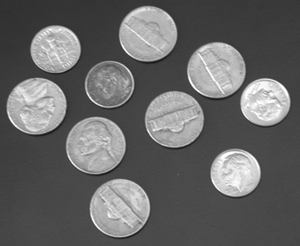
\includegraphics[alt={A greyscale photo of 10 silver coins scattered on a dark grey background.}]{\img/coins.png}\bmlPlusClass{bml_no_invert}
    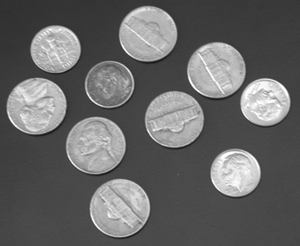
\includegraphics{\img/coins.png}\bmlPlusClass{bml_no_invert}
    \alttext{A greyscale photo of 10 silver coins scattered on a dark grey background.}
    \caption{A PNG image included with \texttt{\textbackslash includegraphics}.}
    \label{fig:coins}
\end{figure}


\subsection{Vector images and diagrams}

\subsubsection{\texttt{tikz} images}
\label{demo:fig:tikz}

Figure~\ref{fig:string} is a \texttt{tikz} diagram included with \verb|\input|.

\begin{figure}[H]
    \centering
    \begin{tikzpicture}[y=0.80pt, x=0.80pt, yscale=-0.7, xscale=0.7, inner sep=0pt, outer sep=0pt]
  \path[draw=black,line join=miter,line cap=round,miter limit=4.00,line
    width=1.200pt] (176.4286,549.5050) .. controls (300.7143,505.2193) and
    (404.2857,517.3622) .. (475.0000,415.2193);
  \path[draw=red,-latex,fill=red,line join=miter,line cap=butt,miter limit=4.00,line
    width=1.200pt] (475.7143,413.0765) -- (507.8571,352.3622);
  \path[draw=red,-latex,fill=red,line join=miter,line cap=butt,miter limit=4.00,line
    width=1.200pt] (174.2857,549.5050) -- (102.1429,571.6479);
  \path[draw=black,dash pattern=on 3.20pt off 3.20pt,line join=miter,line
    cap=butt,miter limit=4.00,line width=0.800pt] (173.5714,548.7908) --
    (97.1429,548.7908);
  \path[draw=black,dash pattern=on 3.20pt off 3.20pt,line join=miter,line
    cap=butt,miter limit=4.00,line width=0.800pt] (476.4286,413.0765) --
    (512.1429,413.0765);
  \path[draw=black,line join=miter,line cap=butt,line width=0.800pt]
    (491.4286,384.5050) .. controls (491.4286,384.5050) and (510.7143,389.5050) ..
    (507.1429,412.3622);
  \path[draw=black,line join=miter,line cap=butt,line width=0.800pt]
    (124.2857,548.0765) .. controls (124.2857,548.0765) and (119.2857,555.9336) ..
    (127.1429,562.3622);
  \path[draw=black,-latex,line join=miter,line cap=butt,miter limit=4.00,line
    width=0.800pt] (88.5714,613.0765) -- (567.1429,613.0765);
  \path[draw=black,dash pattern=on 0.80pt off 1.60pt,line join=miter,line
    cap=butt,miter limit=4.00,line width=0.800pt] (173.5714,549.5050) --
    (173.5714,612.3622);
  \path[draw=black,dash pattern=on 0.80pt off 1.60pt,line join=miter,line
    cap=butt,miter limit=4.00,line width=0.800pt] (475.7143,413.0765) --
    (475.7143,612.3622);
  \path[fill=black] (130.4286,545.0765) node[above right] (text3413)
    {$\theta(x)$};
  \path[fill=black] (490.5714,440.3622) node[above right] (text3417)
    {$\theta(x+dx)$};
  \path[fill=black] (452.8571,636.6479) node[above right] (text3433) {$x+dx$};
  \path[fill=black] (137.8571,582.3622) node[above right] (text3437) {$T$};
  \path[fill=black] (467.7143,386.6479) node[above right] (text3441) {$T$};
  \path[fill=black] (168.7143,636.6479) node[above right] (text3445) {$x$};

\end{tikzpicture}


    \alttext{Diagram of a section of flexible string of length $dx$. Tension is symbolised with a vector T pointing outwards from each end of the string section, at angles theta(x) and theta(x + dx) respectively from the horizontal axis.}
    \caption{Small string element under tension.}
    \label{fig:string}
\end{figure}


\subsection{\texttt{xy} diagrams}
\label{demo:fig:xy}

% The \texttt{tikz-cd} package can also be used to draw commutative diagrams, as an alternative to \texttt{xy}. A \href{https://tikzcd.yichuanshen.de/}{graphical editor is available online}, which generates code. Figure~\ref{fig:cd} shows an example, reproduced from the \href{https://ctan.math.washington.edu/tex-archive/graphics/pgf/contrib/tikz-cd/tikz-cd-doc.pdf}{documentation}.

Figure~\ref{fig:xy} shows an example of a diagram, reproduced from the \href{https://vlmantova.github.io/bookml/#S4.F4}{BookML documentation}.


\begin{figure}
    \begin{bmlimage}
    $$
      \xymatrix{
        U \ar@/_/[ddr]_y \ar@/^/[drr]^x \ar@{.>}[dr]|-{(x,y)} \\
        & X \times_Z Y \ar[d]^q \ar[r]_p & X \ar[d]_f \\
        & Y \ar[r]^g & Z}
    $$
    \end{bmlimage}
    \caption{An example of a \texttt{xymatrix}.}
\end{figure}


\subsubsection{\texttt{pgfplots}}
\label{demo:fig:pgf}

PGF plots are also supported, as shown in Figure~\ref{fig:sqrt}.

\begin{figure}[H]
    \centering
    \begin{tikzpicture}
        \begin{axis}
            \addplot[domain=-3:3, color=blue]{sqrt(x+3)};
        \end{axis}
    \end{tikzpicture}
    \alttext{A plot of sqrt(x+3) between -3 and 3.}
    \caption{Plot created using the \texttt{pgfplots} package.}
    \label{fig:sqrt}
\end{figure}

\subsubsection{SVG}
\label{demo:fig:svg}

Unlike \LaTeX\, HTML can render SVG images directly. If you have SVG images or diagrams as source files, this will produce a clearer image in the HTML version (for example, TikZ images are rendered as SVG). This can be done by using \verb|\iflatexml| to include the SVG image in the HTML version, and the PDF image in the PDF version. This is done below. More information on how this works can be seen in Section~\ref{demo:ifpdf}.

\begin{figure}[H]
    \centering
    \iflatexml
        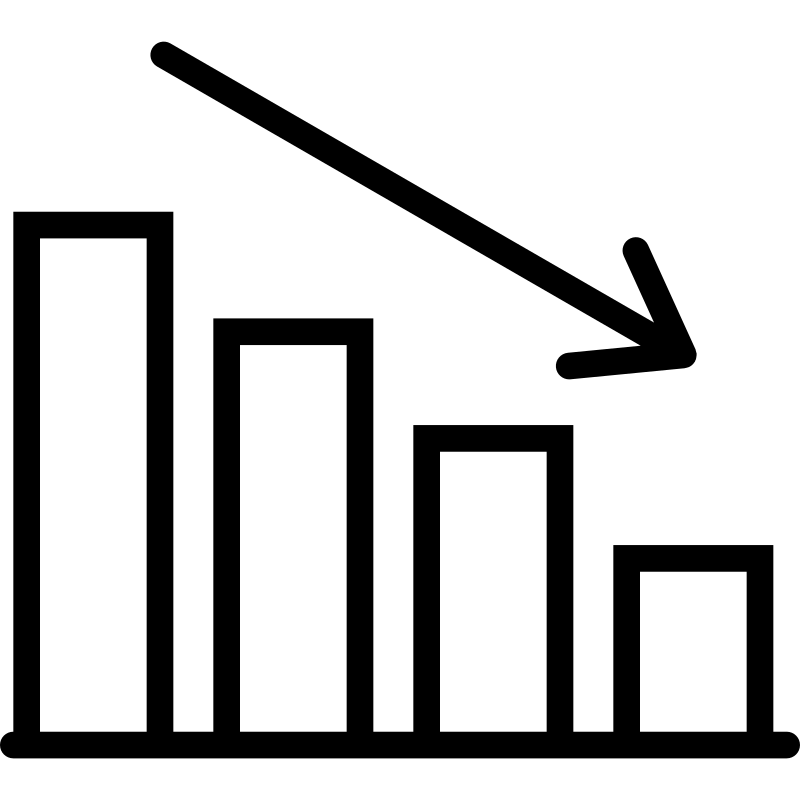
\includegraphics[width=0.25\linewidth]{img/graph.svg}
    \else
        
\includegraphics[width=0.25\linewidth]{img/graph.pdf}
    \fi
    \alttext{Generic bar chart with an arrow to indicate downward trend}
    \label{fig:graph}
\end{figure}



\section{Layout}
\label{demo:layout}

\subsection{Subfigures}
\label{demo:fig:subfig}

The \texttt{subfigure} environment from the \texttt{subcaption} package can be used for both the PDF and HTML versions, as seen in Figure~\ref{fig:subs}. Alternatively, the \texttt{minipage} package can be used, as shown in Figure~\ref{fig:minpage}. Unlike \texttt{subcaption}, \texttt{minipage} forces the figures to be side by side, even if they are too wide to fit on the page. This may be useful if you want to force the figures side by side, but you may wish to swap to \texttt{subcaption} for best flow. 

\begin{figure}[H]
    \centering
    \begin{subfigure}{0.35\textwidth}
        \includegraphics[width=\textwidth]{\img/jcmb.jpg}\bmlPlusClass{bml_no_invert}
        \caption{A JPEG image as a subfigure.}
        \alttext{The main entrance of JCMB.}
        \label{fig:jcmb}
    \end{subfigure}
    \hfill
    \begin{subfigure}{0.6\textwidth}
        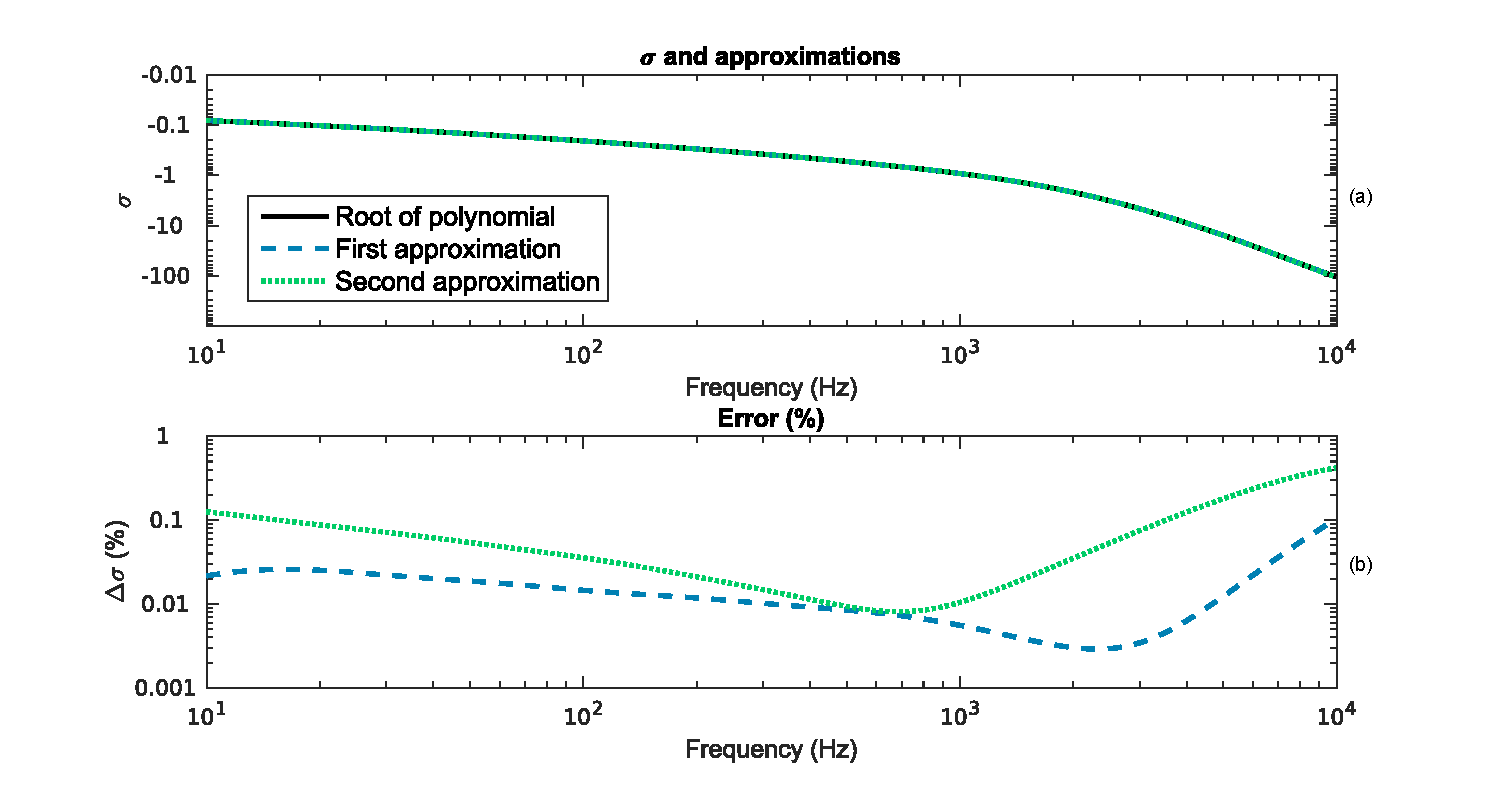
\includegraphics[width=\textwidth]{\img/sigapprox.eps}\bmlPlusClass{bml_no_invert}
        \alttext{Log-log plot showing sigma versus frequency. Three curves overlap almost perfectly: root of polynomial, first approximation, and second approximation.}
        \caption{An EPS file as a subfigure.}
        \label{fig:sig}
    \end{subfigure}
    \caption{Two subfigures,using the \texttt{subcaption} package.}
    \label{fig:subs}
\end{figure}



\begin{figure}[H]
    \centering
    \begin{minipage}{.35\textwidth}
        \centering
        \includegraphics[width=\textwidth]{\img/jcmb.jpg}\bmlPlusClass{bml_no_invert}
        \alttext{The main entrance of JCMB.}
        \caption{A JPEG image as a subfigure.}
        \label{fig:mp-jcmb}
    \end{minipage}%
    \begin{minipage}{0.6\textwidth}
        \centering
        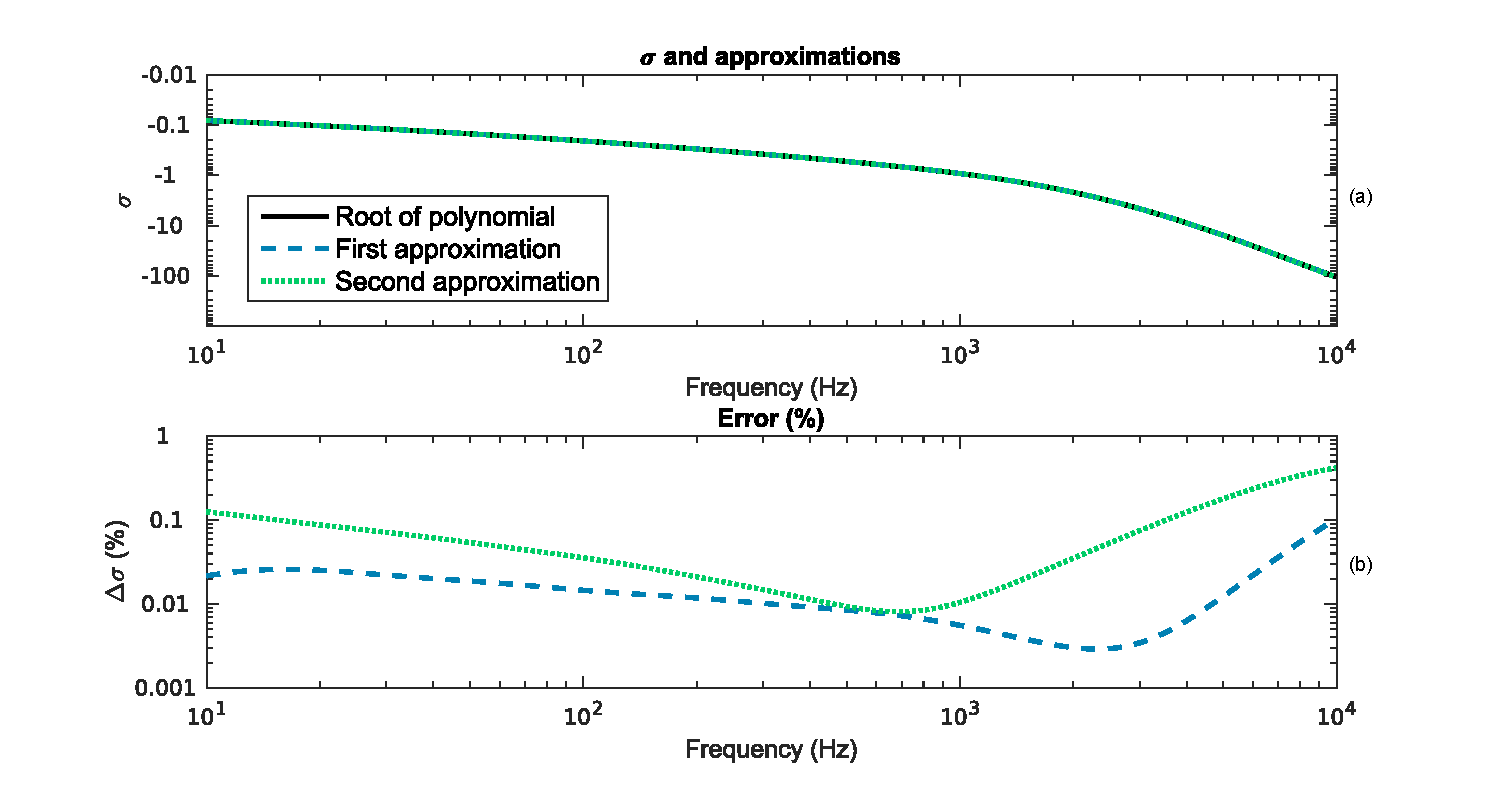
\includegraphics[width=\textwidth]{\img/sigapprox.eps}\bmlPlusClass{bml_no_invert}
        \alttext{Log-log plot showing sigma versus frequency. Three curves overlap almost perfectly: root of polynomial, first approximation, and second approximation.}
        \caption{An EPS file as a subfigure.}
        \label{fig:mp-sig}
    \end{minipage}
    \caption{Two subfigures,using the \texttt{minipage} environment.}
    \label{fig:minpage}
\end{figure}


\subsubsection{Wrapping text around figures}
\label{float:wrap}

\begin{wrapfigure}{r}{0.4\textwidth}
    \centering
    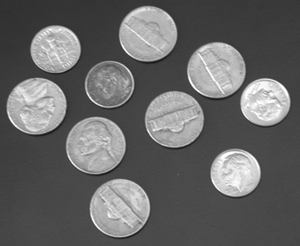
\includegraphics[width=0.35\textwidth]{\img/coins.png}\bmlPlusClass{bml_no_invert}
    \alttext{Photo of 10 silver coins on a dark grey background.}
    \caption{Text wrapped around an image using \texttt{wrapfigure}.}
    \label{fig:wrap}
\end{wrapfigure}

\lipsum[1-2]


\subsection{Tables}
\label{float:tab}

Tables can be typeset using the \texttt{tabular} environment (see Table~\ref{tab:tabular}). Note that the \texttt{tabularx} package is also compatible.

\begin{table}
    \centering
    \begin{tabular}{| l | l | r |} 
      \hline
      cell1 dummy text dummy text dummy text & cell2 & cell3 \\ 
      \hline
      cell1 dummy text dummy text dummy text & cell5 & cell6 \\ 
      \hline
      cell7 & cell8 & cell9 \\ 
      \hline
    \end{tabular}

    \caption{Example table produced with the \texttt{tabular} environment.}
    \label{tab:tabular}
\end{table}


\subsection{Custom floats}
\label{float:custom}

New float types can be created with the \texttt{float} package. For example, Program~\ref{float:prog} is a custom \texttt{program} float (adapted example from the \href{https://en.wikibooks.org/wiki/LaTeX/Floats,_Figures_and_Captions}{LaTeX Wikibooks}). The code is displayed differently but the conversion works.

\begin{program}
  \begin{verbatim}
class HelloWorldApp {
  public static void main(String[] args) {
    //Display the string
    System.out.println("Hello World!");
  }
}
\end{verbatim}
  \caption{The Hello World! program in Java.}
  \label{float:prog}
\end{program}


The package \texttt{multicol} is compatible with BookML, but the in the HTML version, there will not be multiple columns. See bellow, in the PDF version, there are three columns, but in the HTML version, it will be a single column.
\begin{multicols}{3}
     \lipsum[1-2]
\end{multicols}

\section{Other}
\subsection{Multido}
\label{demo:multido}
The \texttt{multido} package is compatible with BookML. It can be used to create loops in your code. For example, the following code will produce a sequence of 8 numbers from 2.00, with a step size of -3.05:

$$
\multido{\n=2.00+-3.05}{8}{\n, }
$$

\subsection{Monospaced output}
\label{demo:code}
The \texttt{listings} package is compatible with BookML. It can be used to create code listings in your document. For example, the following code will produce a listing of a simple Java program:


\begin{lstlisting}[language=Java]
class HelloWorldApp {
  public static void main(String[] args) {
    //Display the string
    System.out.println("Hello World!");
  }
}
\end{lstlisting}
The \texttt{verbatim} environment is also compatible with BookML. It can be used to create verbatim text in your document. For example, the following code will produce a verbatim block of text:

\begin{verbatim}
This is a verbatim block of text.
It will be displayed exactly as it is 
written, with no formatting or special characters such as \LaTeX
\end{verbatim}

\subsection{Referencing from a bibliography}
\label{bib}

The package \texttt{natbib} is compatible with BookML. Note that \texttt{biblatex} is not yet compatible.

This is an example reference~\cite{strikwerda2004}, and another~\citep{parret2016time}. It should not be complex to switch from biblatex to natbib. 


